\documentclass{beamer}
\usetheme{Copenhagen}
\usecolortheme{default}
\usepackage{adjustbox}
\usepackage{fancyvrb}
\usepackage{float}

%Information to be included in the title page:
\title[Gemixque - sistem de recomandări de jocuri video]{Gemixque}
\subtitle{Sistem de recomandări de jocuri video}
\author[Radu Damian]{Radu Damian \and \\[9mm] Dr. Cristian Frăsinaru}

\institute{Facultatea de Informatică}
\date{2022}

\setbeamertemplate{headline}{}
\begin{document}

\frame{\titlepage}


\begin{frame}
  \frametitle{Cuprins}
  \tableofcontents
\end{frame}

\section{Descrierea problemei}
\frame{\tableofcontents[currentsection]}

\begin{frame}{Privirea în ansamblu a problemei}
   Trei elemente principale:
   \begin{itemize}
  \item Utilizatorul
  \item Jocul video
  \item Recenzia
  \end{itemize}
\end{frame}

\begin{frame}{Specificații}
    Fie  \(U \)  mulțimea de utilizatori și \( G \) mulțimea de  jocuri. 
     \[ \forall  u  \in  U,  \;  \exists \; G_u \subseteq  G  \] 
     
     \[ \forall g \in G_u, \; s(u, g) = r_{ug}\]
     
     \[ 1 \leq r_{ug} \leq 10\]
     
    
    
\end{frame}

\begin{frame}{Obiectiv}
\begin{itemize}
  \item Fie \( u \in U \), \(g \notin G_u \) 
  \item \( \hat{s}(u, g) = ?\)
  \end{itemize}
\end{frame}

\section{Neo4j}
\frame{\tableofcontents[currentsection]}
\begin{frame}{Introducere în Neo4j}
    \begin{itemize}
        \item Bază de date NoSQL de tip graf
        \item Datele sunt reținute prin intermediul nodurilor și muchiilor
        \item Utilizează limbajul de interogare Cypher
    \end{itemize}
\end{frame}

\begin{frame}{Caracteristici}
    Un nod are următoarele trăsături:
    
    \begin{itemize}
        \item Reprezintă obiecte/entități
        \item Pot fi etichetate
        \item Pot avea proprietăți
    \end{itemize}
    
    O muchie(relație) este caracterizată de:
    
    \begin{itemize}
        \item Tipul acesteia
        \item Direcția
        \item Poate avea proprietăți
    \end{itemize}
\end{frame}

\begin{frame}[fragile]{Exemplu}
    \begin{figure}[H]
        \centering
        \begin{adjustbox}{max size={\textwidth}{\textheight}}
        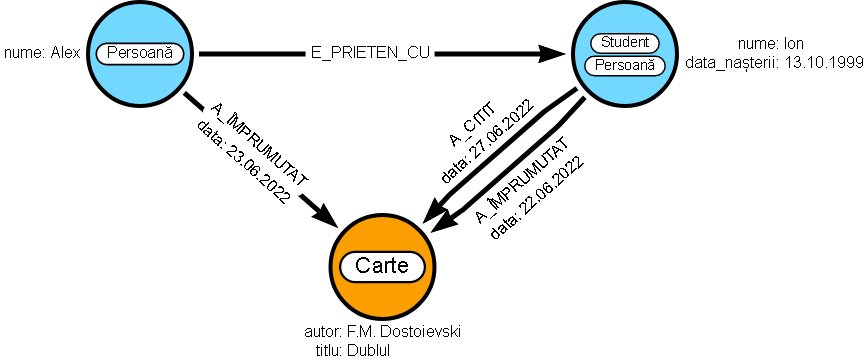
\includegraphics[scale = 0.4]{exemplu_1}
        \end{adjustbox}
    \end{figure}
\end{frame}

\begin{frame}{Limbajul de interogare Cypher}
    \begin{itemize}
        \item inspirat din SQL
        \item prezintă un mod intuitiv de reprezenta noduri și relații prin intermediul unei sintaxe tip ASCII-art
    \end{itemize}
\end{frame}

\begin{frame}{Cypher vs. SQL}
    Studiu de caz:
    \begin{itemize}
        \item modelarea situației din cadrul unei facultăți(studenți, cursuri, profesori)
        \item exemplu interogare în SQL
        \item exemplu interogare în Cypher
        \item conceptul de \emph{pattern-matching}
    \end{itemize}
\end{frame}


\begin{frame}[fragile]{Cypher vs. SQL}
    \centering
    \begin{BVerbatim}
        SELECT p.nume, p.prenume FROM NOTE n 
        JOIN CURSURI c ON n.id_curs = c.id
        JOIN DIDACTIC d ON d.id_curs = c.id
        JOIN PROFESORI p ON p.id = d.id_profesor
        WHERE VALOARE = 10 AND ID_STUDENT = 36;
    \end{BVerbatim}
\end{frame}

\begin{frame}[fragile]{Cypher vs. SQL}
    \begin{figure}[H]
        \centering
        \begin{adjustbox}{max size={\textwidth}{\textheight}}
        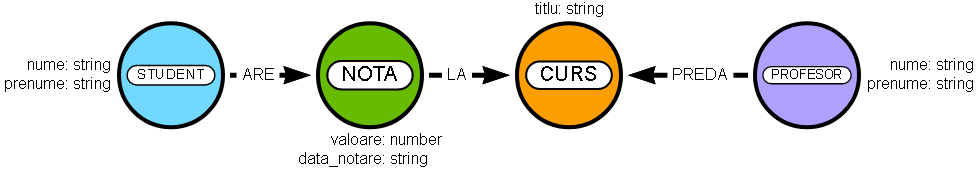
\includegraphics[scale = 0.4]{exemplu_2}
        \end{adjustbox}
    \end{figure}
\end{frame}

\begin{frame}[fragile]{Cypher vs. SQL}
    \centering
    \begin{figure}[H]
\centering
\begin{BVerbatim}
MATCH (s:STUDENT)-[:ARE]->(n:NOTA {valoare: 10}),
(n)-[:LA]->(:CURS)<-[:PREDA]-(p:PROFESOR)
WHERE id(s) = 0
RETURN p.nume, p.prenume
\end{BVerbatim}
\end{figure}
\end{frame}

\begin{frame}{Pattern-matching}
    
\begin{itemize}
    \item Conceptul de \emph{pattern-matching} este introdus prin intermediul clauzei \texttt{MATCH}
    \item În funcție de cum este definit \emph{pattern}-ul în interogare, graful va fi parcurs într-un anumit mod
\end{itemize}

\end{frame}

\begin{frame}[fragile]{Cypher vs. SQL}
    \begin{figure}[H]
        \centering
        \begin{adjustbox}{max size={\textwidth}{\textheight}}
        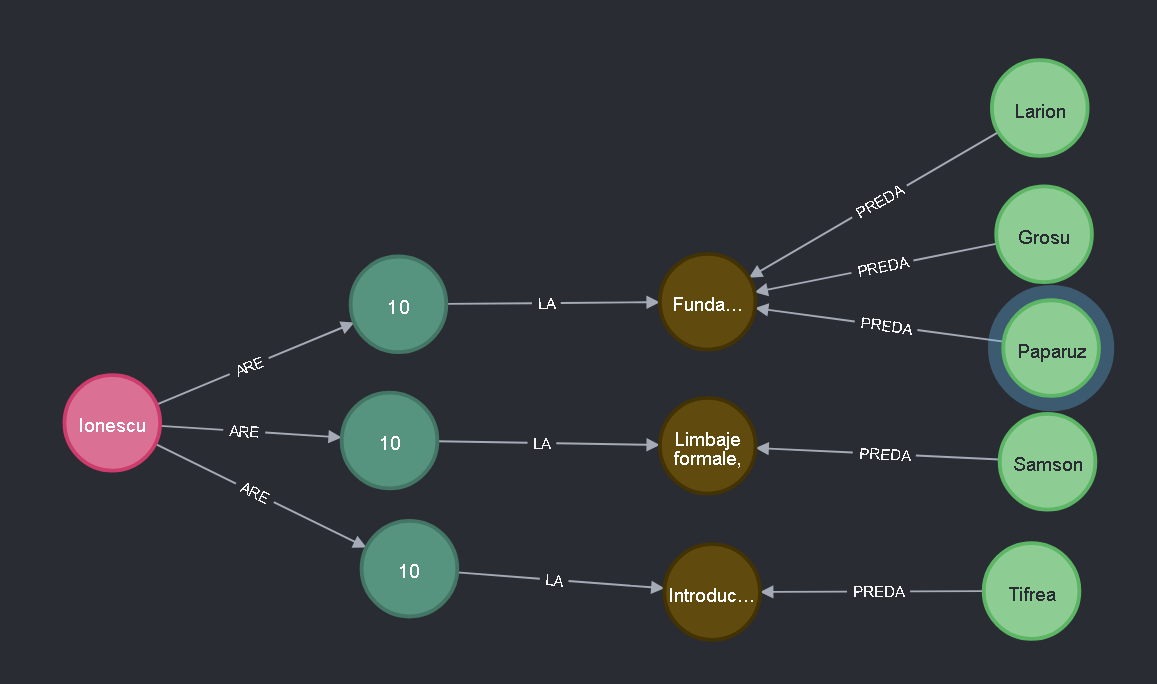
\includegraphics[scale = 0.4]{exemplu_3}
        \end{adjustbox}
    \end{figure}
\end{frame}

\begin{frame}{Schema bazei de date}
    \begin{figure}[H]
        \centering
        \begin{adjustbox}{max size={\textwidth}{\textheight}}
        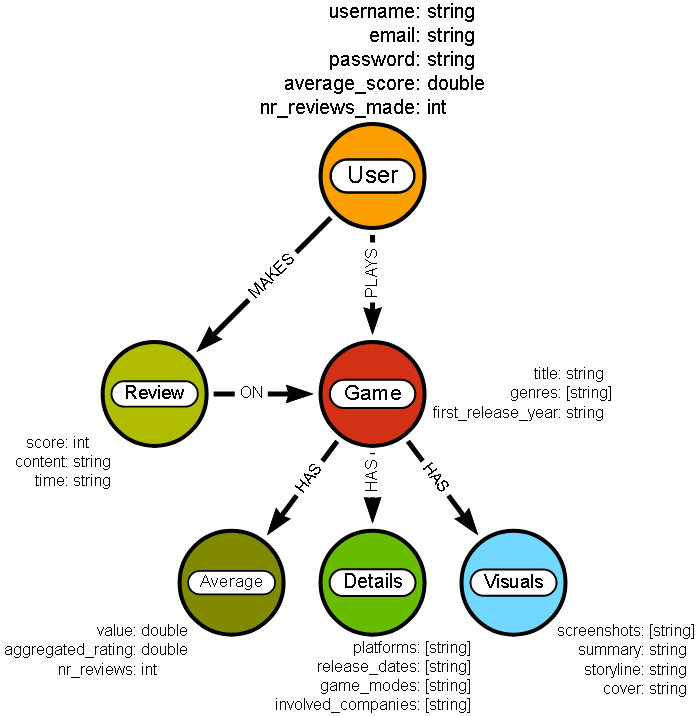
\includegraphics[scale = 0.3]{exemplu_4}
        \end{adjustbox}
    \end{figure}
\end{frame}

\section{Algoritmul de recomandare}
%Contents with current section highlighted
\frame{\tableofcontents[currentsection]}
\begin{frame}{Second section slide}
    test3
\end{frame}

\section{Concluzii}
\frame{\tableofcontents[currentsection]}
\begin{frame}{Concluzii}
	concluzie
\end{frame}

\end{document}